\newpage
\subsubsection{\stid{3.13} CLOVER Sub-project Ginkgo} \label{subsubsect:peeks}
\paragraph{Overview} 
Ginkgo~\footnote{\url{https://github.com/ginkgo-project/ginkgo}} is a modern
linear algebra library engineered towards performance portability, and
productivity. To achieve these goals, the library design is guided by combining
ecosystem extensibility with heavy, architecture-specific kernel optimization
using the platform-native languages CUDA (NVIDIA GPUs), HIP (AMD GPUs), DPC++
(Intel GPUs) and OpenMP (Intel/AMD/ARM multicore). Ginkgo is part of the
extreme-scale Software development Kit (xSDK), part of the Extreme-Scale
Scientific Software Stack (E4S), and has already been integrated as a backend
into simulation libraries like deal.II, MFEM, and HyTeG.
% SUNDIALS, and XGC.



\paragraph{Key Challenges}
% There is a list of challenges to meet with the development of sparse linear
% algebra functionality for the US flagship supercomputers deployed in ECP:
\begin{enumerate}
  \item The extreme levels of hardware concurrency available in the
		GPU-accelerated nodes need to be reflected in fine-grain parallelism in
		the numerical building blocks.
  \item An increasing variety of hardware designs and hardware-native
		programming languages requires a library design that enables platform
		portability without sacrificing performance.
  \item The arithmetic performance of processors growing much faster than the
		memory bandwidth and interconnect speed requires exploring innovative
		strategies for reducing the pressure on all cache/memory levels.
  \item Applications that build upon the fast solution of many independent
		moderate-sized sparse linear systems require batched sparse linear
		algebra functionality.
  \item Applications building upon matrix-free methods requires the flexibility
		to compose linear solvers out of library-native and customized external
		functionality.
\end{enumerate}

\begin{figure}[!h]
\centering
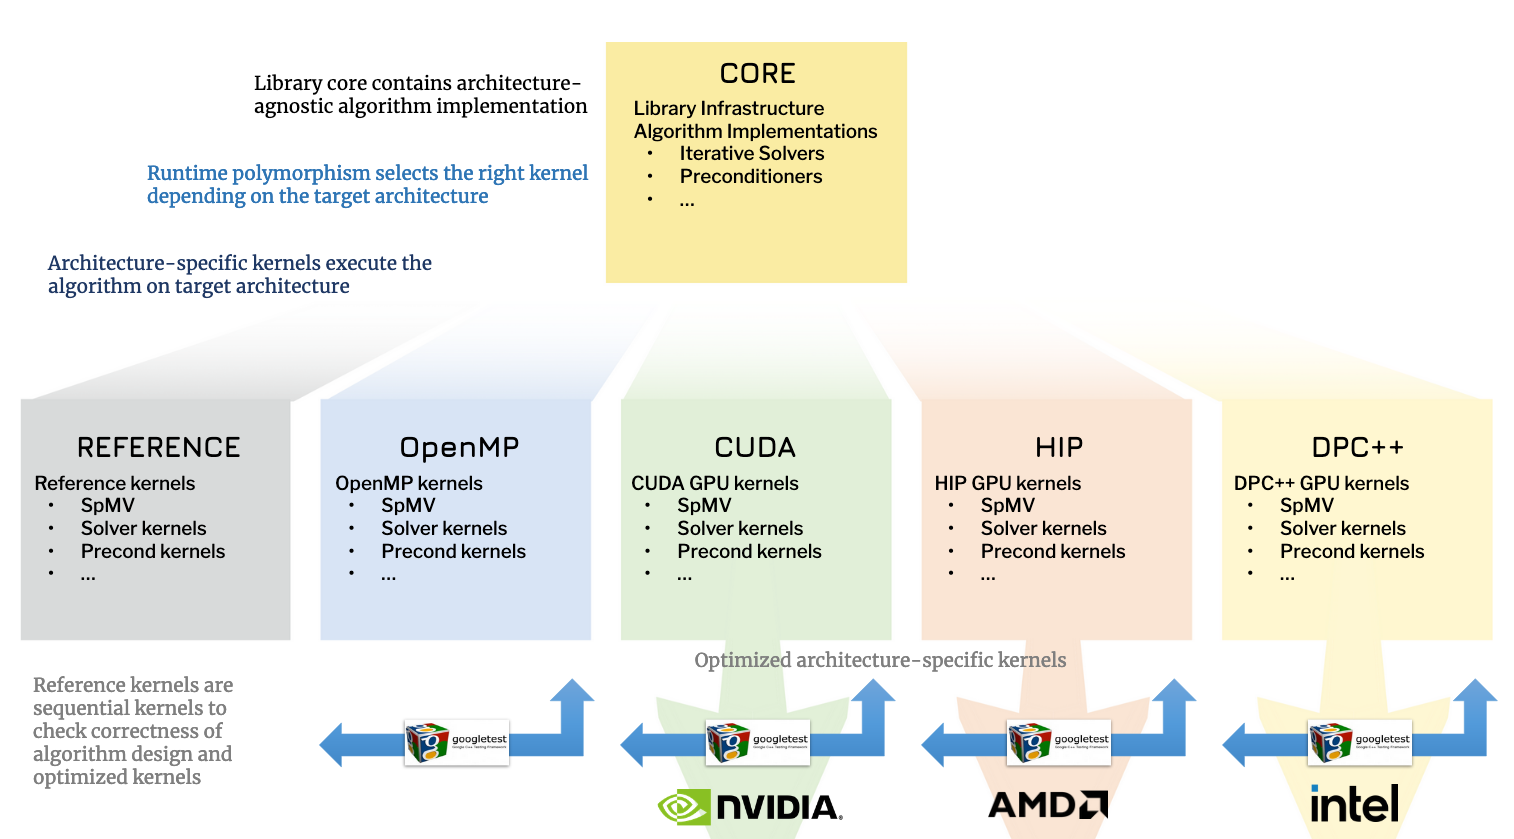
\includegraphics[width=.8\columnwidth]{projects/2.3.3-MathLibs/2.3.3.13-CLOVER/ginkgo_portability_crop}
\caption{\label{fig:ginkgoportability}The portability design of the Ginkgo math
  library enables high performance kernel implementations in the vendor-supported
  programming language.}
\end{figure}


\paragraph{Solution Strategy}

The Ginkgo team is addressing these challenges by striving for platform
portability, modularity, extensibility, and hardware-aware algorithm design.

\begin{enumerate}
  \item \textbf{Architecture-portable software design:}
		Ginkgo~\cite{anzt2020ginkgo} employs a design that decouples the
		algorithm implementations from the hardware-specific kernel
		implementations, thereby acknowledging the importance of platform
		portability and allowing for architecture-specific kernel optimization
		in the vendor language, see Figure~\ref{fig:ginkgoportability}.
  \item \textbf{Modularity, flexibility, and extensibility:} Ginkgo employs a
		``linear operator'' abstraction for all functionality, which allows for
		flexibility in combining functionality and interfacing external
		operators.
  \item \textbf{Sustainability efforts:} Ginkgo adheres the Better Scientific
		Software (BSSw) design principles~\cite{betterscientificsoftware} that
		ensure production-quality code by featuring unit testing, automated
		configuration and installation, Doxygen code documentation, as well as a
		continuous integration and continuous benchmarking
		framework~\cite{pasc_anzt}. Ginkgo is an open source effort licensed
		under the BSD 3-clause and included in the xSDK and E4S software
		packages.
  \item \textbf{Fine-grain parallelism:} Ginkgo features linear algebra
		building blocks and advanced algorithms for preconditioning and solving
		linear systems that can efficiently leverage the concurrency of modern
		GPUs, including (incomplete) parallel factorizations, parallel sparse
		triangular solves, parallel matrix operations, and parallel iterative
		methods.
  \item \textbf{Mixed precision methods:} Ginkgo features a memory accessor
		that encapsulates on-the-fly compression for decoupling the memory
		precision from the arithmetic precision. This allows accelerating
		memory-bound algorithms that can compensate or tolerate some information
		loss in the memory operations. The memory accessor can also be used to
		increase the result accuracy of memory-bound kernels that benefit from
		using a more complex precision format in the arithmetic operations
		without performance loss.
  \item \textbf{Batched preconditioned iterative solvers:} Ginkgo contains high
		performance batched iterative solvers that handle the concurrent
		solution of a set of independent sparse linear systems of moderate size.
		The batched iterative solvers allow for some flexibility in terms of the
		preconditioner and monitor the system-individual convergence without
		performance degradation.
\end{enumerate}

\paragraph{Recent Progress}
\begin{enumerate}
  \item The Ginkgo library realized native support for Intel GPUs (via
		DPC++)~\cite{tsai2021porting}.
  \item MFEM treating Ginkgo as numerical backend allows accelerating MFEM
		simulations with AMD GPUs, Intel GPUs, and NVIDIA GPUs.
  \item The Ginkgo library has been expanded with new advanced preconditioners
		such as ISAI and Multigrid, also supporting mixed-precision capabilities~\cite{10.1007/978-3-030-85665-6_34}.
  \item Based on the memory accessor, the Ginkgo team deployed a Compressed
		Basis GMRES (CB-GMRES) solver that outperforms the standard GMRES solver
		by storing the Krylov basis vectors in lower precision, therewith
		accelerating the memory access~\cite{DBLP:journals/corr/abs-2009-12101}.
  \item The Ginkgo team successfully employed the batched iterative solvers for
		the hydrodynamic problems arising in the PeleLM
		simulations and the gyrokinetic problems arising in the
		XGC simulations.
\end{enumerate}


\paragraph{Next Steps}
Our next efforts are:
\begin{enumerate}
  \item \textbf{Deployment of multi-node functionality:} Ginkgo already has
		experimental support for multi-node execution via an executor-agnostic
		MPI layer. We will extend the support and make it production-ready.
  \item \textbf{Deployment of GPU-resident spare direct solvers:} In response to
		an urgent need of national power grid simulations, we will develop
		GPU-resident sparse direct solvers.
  \item \textbf{Block-versions of the parallel Incomplete factorization
		preconditioner:} To better reflect the properties of the ECP application
		projects, we will deploy blocked versions of the ParILU and ParILUT
		parallel ILU and parallel threshold ILU preconditioners in the Ginkgo
		software library.
  \item \textbf{Problem-specific preconditioners for MFEM:} In collaboration
		with the ECP CEED cluster, we will design problem-specific mixed
		precision preconditioners for matrix-free finite element simulations.
\end{enumerate}
